\documentclass[a4paper,12pt]{article} 
%Packages included by Soon Chee Loong, TODO 
\usepackage{amssymb}  % For \therefore
\usepackage{fullpage} % Package to use full page
\usepackage{parskip} % Package to tweak paragraph skipping
\usepackage{tikz} % Package for drawing
\usepackage{hyperref}
\usepackage{palatino}
\usepackage{minted} % For code highlighting 
\usepackage{amsmath} % To split long equations
% For sketching graphs 
\usetikzlibrary{bayesnet}
% More custom packages (default or by Christopher) 
\usepackage{amssymb}
\usepackage{caption} % To control caption properties
\usepackage{multirow} % Used to merge multiple tables cells along a row
\usepackage{mathtools} % Double vertical bars for norms
\usepackage{physics} % Partial derivatives
\usepackage{bm} % For bold Greek letters
\usepackage{subcaption}  % For \subfigures environment and \subfloat method
\usepackage{wrapfig} % To warp figures
\usepackage{tabularx}
\usepackage{tabulary} % To create tables that wrap texts
\usepackage{booktabs}
\usepackage{relsize}
\usepackage{cite}
%------------------------------------------------------------------
% Adjust line spacing
\renewcommand{\baselinestretch}{1.5}
%------------------------------------------------------------------
\DeclareMathOperator*{\argmin}{arg\,min}
\DeclareMathOperator*{\argmax}{arg\,max}

% Custom commands
\newcommand{\given}{\ | \ }
\newcommand{\x}{\mathbf{x}}
\newcommand{\X}{\mathbf{X}}
\newcommand{\means}{\bm{\mu}}
\newcommand{\cov}{\mathbf{\Sigma}}
\newcommand{\ident}{\mathbf{I}_D}
\newcommand{\gradmu}{\nabla_{\bm{\mu}}}
\newcommand{\msgNtoF}[2]{\mu_{#1 \rightarrow f_{#2}}(#1)}
\newcommand{\msgFtoN}[2]{\mu_{f_{#1} \rightarrow #2}(#2)}
\newcommand{\msgFtoNCond}[3]{\mu_{f_{#1} \rightarrow #2}(#2 \given #3)}
\newcommand{\factorChris}[2]{f_{#1 #2}(#1, #2)}
%------------------------------------------------------------------
% For independence and non independence notation
\usepackage{slashed}
\newcommand{\ci}{\perp\!\!\!\perp}
\newcommand{\nci}{\slashed{\ci}}
%------------------------------------------------------------------
% Colour Definitions
\definecolor{blue}{HTML}{1f77b4}
\definecolor{orange}{HTML}{ff7f0e}
\definecolor{green}{HTML}{2ca02c}
\definecolor{red}{HTML}{d62728}
\definecolor{purple}{HTML}{9467bd}
\definecolor{bg}{rgb}{0.95, 0.95, 0.95}

%------------------------------------------------------------------
% For subsubsubsection  & paragraph definition

\usepackage{titlesec}
\titleclass{\subsubsubsection}{straight}[\subsection]

\newcounter{subsubsubsection}[subsubsection]

\renewcommand\thesubsubsubsection{\thesubsubsection.\arabic{subsubsubsection}}
\renewcommand\theparagraph{\thesubsubsubsection.\arabic{paragraph}}
\renewcommand\thesubparagraph{\theparagraph.\arabic{subparagraph}}

\titleformat{\subsubsubsection}
  {\normalfont\normalsize\bfseries}{\thesubsubsubsection}{1em}{}
\titlespacing*{\subsubsubsection}
{0pt}{3.25ex plus 1ex minus .2ex}{1.5ex plus .2ex}

\makeatletter
\renewcommand\paragraph{\@startsection{paragraph}{5}{\z@}%
  {3.25ex \@plus1ex \@minus.2ex}%
  {-1em}%
  {\normalfont\normalsize\bfseries}}
\renewcommand\subparagraph{\@startsection{subparagraph}{6}{\parindent}
  {3.25ex \@plus1ex \@minus .2ex}%
  {-1em}%
  {\normalfont\normalsize\bfseries}}
\def\toclevel@subsubsubsection{4}
\def\toclevel@paragraph{5}
\def\toclevel@paragraph{6}
\def\l@subsubsubsection{\@dottedtocline{4}{7em}{4em}}
\def\l@paragraph{\@dottedtocline{5}{10em}{5em}}
\def\l@subparagraph{\@dottedtocline{6}{14em}{6em}}
\@addtoreset{subsubsubsection}{section}
\@addtoreset{subsubsubsection}{subsection}
\@addtoreset{paragraph}{subsubsubsection}
\makeatother

\setcounter{secnumdepth}{6}
\setcounter{tocdepth}{6}

%------------------------------------------------------------------
% Collaboration Notes 
% 0. Ensure tex always compiles, fix any errors immediately
%		This doesn't have version control. So don't mess up.  
% 1. Work on 1 main.tex file only 
% 	Easier to back-up to local
% 	Easier to work on local if needed. 
% 2. TODO: Mark anything important to do as TODO
% 	so we can easily search for all TODO: comments before submitting. 
%------------------------------------------------------------------
\title{ECE521 Winter 2017: Assignment 4}
\author{FuYuan Tee, (999295837)
  \thanks{Equal Contribution (50\%), fuyuan.tee@mail.utoronto.ca}
\and Chee Loong Soon, (999295793) \thanks{Equal Contribution (50\%),  cheeloong.soon@mail.utoronto.ca}} 
\date{April 9th, 2017}
\begin{document}
\maketitle
\tableofcontents
\clearpage

%------------------------------------------------------------------
\section{Graphical Models}
\subsection{Graphical models from factorization}

\begin{equation}
\label{equation:JointDist}
\begin{split}
P(a,b,c,d,e,f,) = P(a|b)P(b)P(c|a,b)P(d|b)P(e|c)P(f|b,e) \\
=  P(f|b,e)P(e|c)P(c|a,b)P(a|b)P(d|b)P(b)
\end{split}
\end{equation}

\subsubsection{Sketch Bayesian Networks}
Bayesian Network corresponding to joint distribution \ref{equation:JointDist}.

\begin{figure}[!htb]
\centering
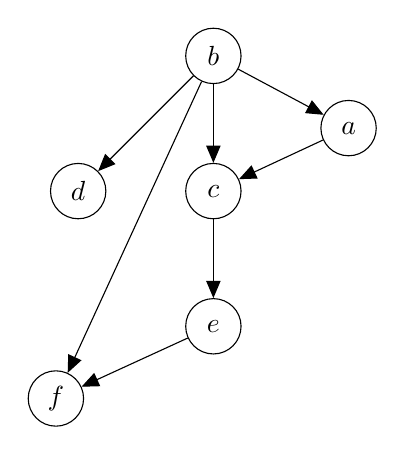
\begin{tikzpicture}
  % Define nodes
  \node[latent]             (b) {$b$};
  \node[latent, below=of b] (c) {$c$};
  \node[latent, right=of c, yshift=0.8cm] (a) {$a$};
  \node[latent, left=of c] (d) {$d$};
  \node[latent, below=of c] (e) {$e$};
  \node[latent, below=of e, xshift=-2.0cm, yshift=0.8cm] (f) {$f$};
  % Connect nodes
  \edge {b} {c};
  \edge {b} {a};
  \edge {b} {d};
  \edge {a} {c};
  \edge {c} {e};
  \edge {b} {f};
  \edge {e} {f};
\end{tikzpicture}
\end{figure}

\clearpage

\subsubsection{Sketch Factor Graph}
Factor Graph corresponding to joint distribution \ref{equation:JointDist}.

\begin{figure}[!htb]
\centering
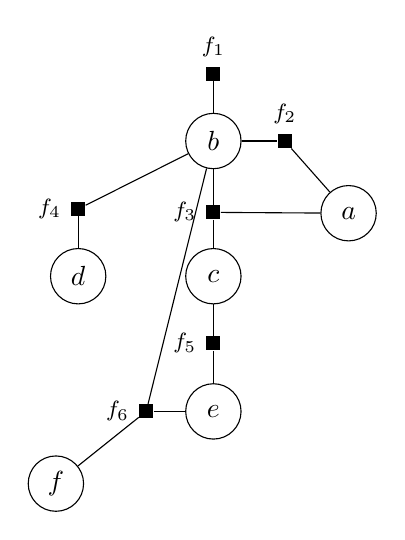
\begin{tikzpicture}
\label{fig:factorGraphA}
  % Define nodes
  \node[latent]             (b) {$b$};
  \node[latent, below=of b] (c) {$c$};
  \node[latent, right=of c, yshift=0.8cm] (a) {$a$};
  \node[latent, left=of c] (d) {$d$};
  \node[latent, below=of c] (e) {$e$};
  \node[latent, below=of e, xshift=-2.0cm, yshift=0.8cm] (f) {$f$};
  % Define factors 
  \factor[above=of b] {factor1} {$f_1$} {} {};
  \factor[above=of a, right=of b, xshift=1.5] {factor2} {$f_2$} {} {};
  \factor[above=of c, below=of b, yshift=-1.5] {factor3} {left:$f_3$} {} {};
  \factor[above=of d] {factor4} {left:$f_4$} {} {};
  \factor[above=of e, below=of c] {factor5} {left:$f_5$} {} {};
  \factor[below=of e, left=of e] {factor6} {left:$f_6$} {} {};
  % Define factor edges 
  \factoredge[-] {b} {factor1} {};
  \factoredge[-] {b} {factor2} {a};
  \factoredge[-] {b} {factor3} {a,c};
  \factoredge[-] {b} {factor4} {d};
  \factoredge[-] {c} {factor5} {e};
  \factoredge[-] {b} {factor6} {e,f};
\end{tikzpicture}
\end{figure}

The factors with corresponding distribution are shown in \ref{equation:FactorOneOneTwo}.
\begin{equation}
\label{equation:FactorOneOneTwo}
\begin{split}
f_{1}(b) & = P(b) \\
f_{2}(a,b) & = P(a|b) \\
f_{3}(a,b,c) & = P(c|a,b) \\
f_{4}(b,d) & = P(d|b) \\
f_{5}(c,e) & = P(e|c) \\
f_{6}(b,e,f) & = P(f|b,e) 
\end{split}
\end{equation}

\clearpage 

According to ECE521 Winter 2017 Tutorial 8 page 33, 
this can be simplified to

\begin{figure}[!htb]
\centering
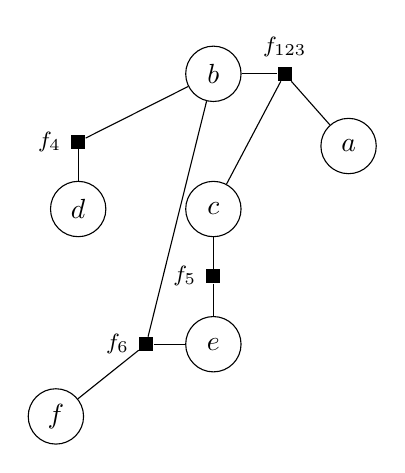
\begin{tikzpicture}
\label{fig:factorGraphA}
  % Define nodes
  \node[latent]             (b) {$b$};
  \node[latent, below=of b] (c) {$c$};
  \node[latent, right=of c, yshift=0.8cm] (a) {$a$};
  \node[latent, left=of c] (d) {$d$};
  \node[latent, below=of c] (e) {$e$};
  \node[latent, below=of e, xshift=-2.0cm, yshift=0.8cm] (f) {$f$};
  % Define factors 
  \factor[above=of a, right=of b, xshift=1.5] {factor123} {$f_{123}$} {} {};
  \factor[above=of d] {factor4} {left:$f_4$} {} {};
  \factor[above=of e, below=of c] {factor5} {left:$f_5$} {} {};
  \factor[below=of e, left=of e] {factor6} {left:$f_6$} {} {};
  % Define factor edges 
  \factoredge[-] {b} {factor123} {a,c};
  \factoredge[-] {b} {factor4} {d};
  \factoredge[-] {c} {factor5} {e};
  \factoredge[-] {b} {factor6} {e,f};
\end{tikzpicture}
\end{figure}

The factors with corresponding distribution corresponding to the simplified Factor Graph shown in equation \ref{equation:FactorSimplified}.
\begin{equation}
\label{equation:FactorSimplified}
\begin{split}
f_{123}(a,b,c) & = P(c|a,b) P(a|b)P(b)  \\
f_{4}(b,d) & = P(d|b) \\
f_{5}(c,e) & = P(e|c) \\
f_{6}(e,f) & = P(f|b,e) 
\end{split}
\end{equation}

\clearpage

\subsubsection{Sketch Markov Random Field}

\begin{figure}[!htb]
\centering
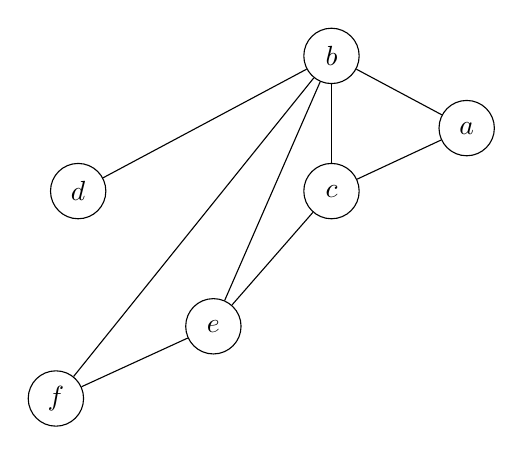
\begin{tikzpicture}
  % Define nodes
  \node[latent]             (b) {$b$};
  \node[latent, below=of b] (c) {$c$};
  \node[latent, right=of c, yshift=0.8cm] (a) {$a$};
  \node[latent, left=of c, xshift=-1.5cm] (d) {$d$};
  \node[latent, below=of c, xshift=-1.5cm] (e) {$e$};
  \node[latent, below=of e, xshift=-2.0cm, yshift=0.8cm] (f) {$f$};
  % Connect nodes
  \edge[-] {b} {c};
  \edge[-] {b} {a};
  \edge[-] {b} {d};
  \edge[-] {a} {c};
  \edge[-] {c} {e};
  \edge[-] {b} {f};
  \edge[-] {e} {f};
  \edge[-] {b} {e};
\end{tikzpicture}
\end{figure}

The equations are shown in \ref{equation:MarkovRandom}. The parameters to each maximum cliques are the vertex to each maximal clique. 

\begin{equation}
\label{equation:MarkovRandom}
\begin{split}
\psi_{1}(a,b,c) &= P(c|a,b)P(a|b)P(b) \\
\psi_{2}(b,c,e) &=  P(e|c) \\
\psi_{3}(b,e,f) &= P(f|b,e) \\
\psi_{4}(b,d) &= P(d|b) \\
\end{split}
\end{equation}

\clearpage
%------------------------------------------------------------------
\subsection{Conversion between graphical models}

\subsubsection{Factor Graph}

Factor Graph $(a)$   
\begin{figure}[!htb]
\centering
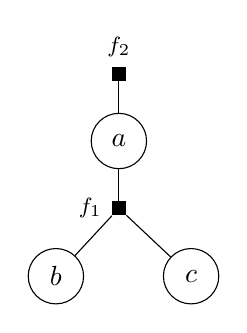
\begin{tikzpicture}
  % Define nodes
  \node[latent]             (b) {$b$};
  \node[latent, above=of b, xshift=0.8cm] (a) {$a$};
  \node[latent, right=of b]       (c) {$c$};
  \factor[below=of a] {factor1} {left:$f_1$} {} {};
  \factor[above=of a] {factor2} {$f_2$} {} {};
  \factoredge[-] {a} {factor1} {b,c};
  \factoredge[-] {a} {factor2} {};
  % Connect the nodes
\end{tikzpicture}
\end{figure}

The conditional independence properties for Factor Graph $(a)$ are
%
\begin{equation}
\label{equation:conditionalIndependenceA}
\begin{split}
b \nci c | a \\
a \nci b | c \\
a \nci c | b 
\end{split}
\end{equation}
%
\begin{figure}[!htb]
\centering
\begin{subfigure}[t]{0.3\textwidth}
	\centering
    \caption*{$b \nci c | a$}
	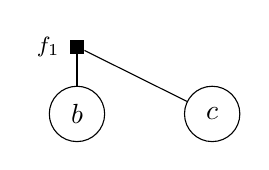
\begin{tikzpicture}
      % Define nodes
      \node[latent]             (b) {$b$};
      \node[latent, right=of b]       (c) {$c$};
      \factor[above=of b] {factor1} {left:$f_1$} {} {};
      \factoredge[-] {b} {factor1} {c};
      % Connect the nodes
	\end{tikzpicture}
\end{subfigure}
\begin{subfigure}[t]{0.3\textwidth}
	\centering
    \caption*{$a \nci b | c$}
    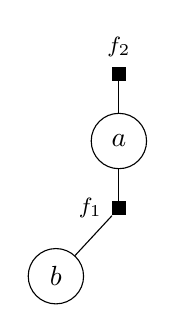
\begin{tikzpicture}
      % Define nodes
      \node[latent]             (b) {$b$};
      \node[latent, above=of b, xshift=0.8cm] (a) {$a$};
      \factor[below=of a] {factor1} {left:$f_1$} {} {};
      \factor[above=of a] {factor2} {$f_2$} {} {};
      \factoredge[-] {a} {factor1} {b};
      \factoredge[-] {a} {factor2} {};
      % Connect the nodes
    \end{tikzpicture}
\end{subfigure}
\begin{subfigure}[t]{0.3\textwidth}
	\centering
    \caption*{$a \nci c | b$}
    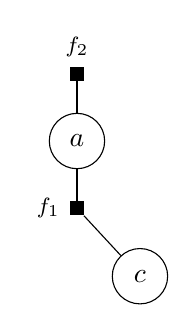
\begin{tikzpicture}
      % Define nodes
      \node[latent] (a) {$a$};
      \node[latent, below=of a, xshift=0.8cm] (c) {$c$};
      \factor[below=of a] {factor1} {left:$f_1$} {} {};
      \factor[above=of a] {factor2} {$f_2$} {} {};
      \factoredge[-] {a} {factor1} {c};
      \factoredge[-] {a} {factor2} {};
      % Connect the nodes
    \end{tikzpicture}
\end{subfigure}
\end{figure}

\clearpage

Factor Graph $(b)$
%
\begin{figure}[!htb]
\centering
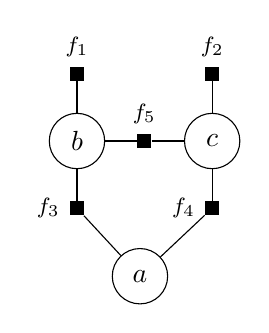
\begin{tikzpicture}
  % Define nodes
  \node[latent]               (b) {$b$};
  \node[latent, right=of b]         (c) {$c$};
  \node[latent, below=of b, xshift=0.8cm] (a) {$a$};
  \factor[above=of b] {factor1} {$f_1$} {} {};
  \factor[above=of c] {factor2} {$f_2$} {} {};
  \factor[below=of b] {factor3} {left:$f_3$} {} {};
  \factor[below=of c] {factor4} {left:$f_4$} {} {};
  \factor[right=of b] {factor5} {$f_5$} {} {};
  \factoredge[-] {b} {factor3} {a};
  \factoredge[-] {c} {factor4} {a};
  \factoredge[-] {b} {factor5} {c};
  \factoredge[-] {b} {factor1} {};
  \factoredge[-] {c} {factor2} {};
\end{tikzpicture}
\end{figure}

The conditional independence properties for Factor Graph $b)$ are
%
\begin{equation}
\label{equation:conditionalIndependenceB}
\begin{split}
b \nci c | a \\
a \nci b | c \\
a \nci c | b 
\end{split}
\end{equation}
%
\begin{figure}[!htb]
\centering
\begin{subfigure}[t]{0.3\textwidth}
	\centering
    \caption*{$b \nci c | a$}
    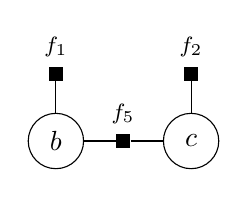
\begin{tikzpicture}
      % Define nodes
      \node[latent]               (b) {$b$};
      \node[latent, right=of b]         (c) {$c$};
      \factor[above=of b] {factor1} {$f_1$} {} {};
      \factor[above=of c] {factor2} {$f_2$} {} {};
      \factor[right=of b] {factor5} {$f_5$} {} {};
      \factoredge[-] {b} {factor5} {c};
      \factoredge[-] {b} {factor1} {};
      \factoredge[-] {c} {factor2} {};
    \end{tikzpicture}
\end{subfigure}
\begin{subfigure}[t]{0.3\textwidth}
	\centering
    \caption*{$a \nci b | c$}
    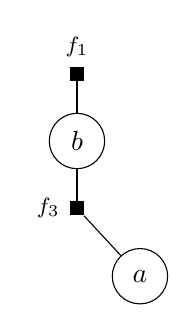
\begin{tikzpicture}
      % Define nodes
      \node[latent]               (b) {$b$};
      \node[latent, below=of b, xshift=0.8cm] (a) {$a$};
      \factor[above=of b] {factor1} {$f_1$} {} {};
      \factor[below=of b] {factor3} {left:$f_3$} {} {};
      \factoredge[-] {b} {factor3} {a};
      \factoredge[-] {b} {factor1} {};
    \end{tikzpicture}
\end{subfigure}
\begin{subfigure}[t]{0.3\textwidth}
	\centering
    \caption*{$a \nci c | b$}
    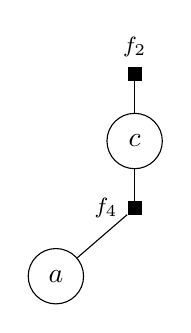
\begin{tikzpicture}
      % Define nodes
      \node[latent] (a) {$a$};
      \node[latent, above=of a, xshift=1.0cm]         (c) {$c$};
      \factor[above=of c] {factor2} {$f_2$} {} {};
      \factor[below=of c] {factor4} {left:$f_4$} {} {};
      \factoredge[-] {c} {factor4} {a};
      \factoredge[-] {c} {factor2} {};
    \end{tikzpicture}
\end{subfigure}
\end{figure}

\clearpage 

%------------------------------------------------------------------
\subsubsubsection{Factor Graph to BN}

\paragraph{Factor Graph (a) to BN}
Converting to Bayesian Networks while maintaining conditional independence in \ref{equation:conditionalIndependenceA} has two different solutions according to conversion rules given in class.  

Solution 1:
\begin{figure}[!htb]
\centering
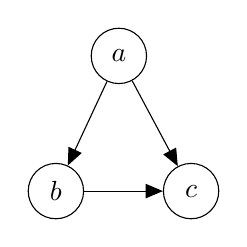
\begin{tikzpicture}
  % Define nodes
  \node[latent]             (b) {$b$};
  \node[latent, above=of b, xshift=0.8cm] (a) {$a$};
  \node[latent, right=of b]       (c) {$c$};
  % Connect nodes
  \edge {a} {b};
  \edge {a} {c};
  \edge {b} {c};
\end{tikzpicture}
\end{figure}
%
\begin{equation}
\label{equation:conditionalIndependenceBNaSolution1}
\begin{split}
P(a,b,c) = P(c|a,b)P(b|a)P(a) = \frac{1}{Z} f_{1}(a,b,c)f_{2}(a) \\
Z = \sum_{a,b,c} f_{1}(a,b,c)f_{2}(a) \\
\end{split}
\end{equation}
%
\begin{figure}[!htb]
\centering
\begin{subfigure}[t]{0.3\textwidth}
	\centering
    \caption*{$b \nci c | a$}
    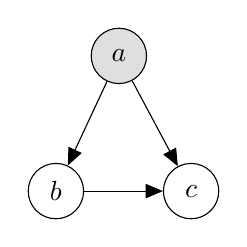
\begin{tikzpicture}
      % Define nodes
      \node[latent]             (b) {$b$};
      \node[latent, obs, above=of b, xshift=0.8cm] (a) {$a$};
      \node[latent, right=of b]       (c) {$c$};
      % Connect nodes
      \edge {a} {b};
      \edge {a} {c};
      \edge {b} {c};
    \end{tikzpicture} \\
    Cascade from b to c
\end{subfigure}
\begin{subfigure}[t]{0.3\textwidth}
	\centering
    \caption*{$a \nci b | c$}
    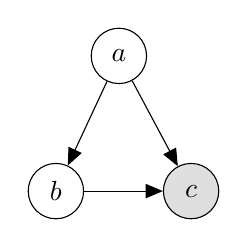
\begin{tikzpicture}
      % Define nodes
      \node[latent]             (b) {$b$};
      \node[latent, above=of b, xshift=0.8cm] (a) {$a$};
      \node[latent, obs, right=of b]       (c) {$c$};
      % Connect nodes
      \edge {a} {b};
      \edge {a} {c};
      \edge {b} {c};
    \end{tikzpicture} \\
    Cascade from a to b. V-structure from c to a and b.
\end{subfigure}
\begin{subfigure}[t]{0.3\textwidth}
	\centering
    \caption*{$a \nci c | b$}
    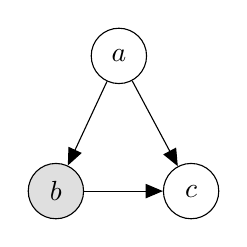
\begin{tikzpicture}
      % Define nodes
      \node[latent, obs]             (b) {$b$};
      \node[latent, above=of b, xshift=0.8cm] (a) {$a$};
      \node[latent, right=of b]       (c) {$c$};
      % Connect nodes
      \edge {a} {b};
      \edge {a} {c};
      \edge {b} {c};
    \end{tikzpicture} \\
    Cascade from a to c
\end{subfigure}
\end{figure}

\clearpage

Solution 2:
\begin{figure}[!htb]
\centering
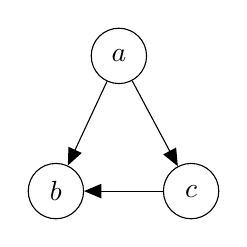
\begin{tikzpicture}
  % Define nodes
  \node[latent]             (b) {$b$};
  \node[latent, above=of b, xshift=0.8cm] (a) {$a$};
  \node[latent, right=of b]       (c) {$c$};
  % Connect nodes
  \edge {a} {b};
  \edge {a} {c};
  \edge {c} {b};
\end{tikzpicture}
\end{figure}
%
\begin{equation}
\label{equation:conditionalIndependenceBNaSolution2}
\begin{split}
P(a,b,c) = P(b|a,c)P(c|a)P(a) = \frac{1}{Z} f_{1}(a,b,c)f_{2}(a) \\
Z = \sum_{a,b,c} f_{1}(a,b,c)f_{2}(a) \\
\end{split}
\end{equation}
%
\begin{figure}[!htb]
\centering
\begin{subfigure}[t]{0.3\textwidth}
	\centering
    \caption*{$b \nci c | a$}
    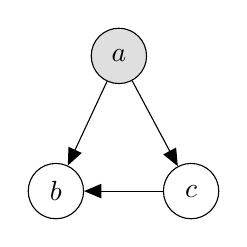
\begin{tikzpicture}
      % Define nodes
      \node[latent]             (b) {$b$};
      \node[latent, obs, above=of b, xshift=0.8cm] (a) {$a$};
      \node[latent, right=of b]       (c) {$c$};
      % Connect nodes
      \edge {a} {b};
      \edge {a} {c};
      \edge {c} {b};
    \end{tikzpicture} \\
    Cascade from c to b
\end{subfigure}
\begin{subfigure}[t]{0.3\textwidth}
	\centering
    \caption*{$a \nci b | c$}
    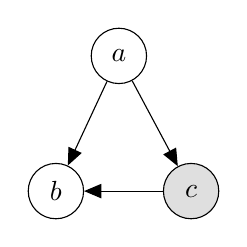
\begin{tikzpicture}
      % Define nodes
      \node[latent]             (b) {$b$};
      \node[latent, above=of b, xshift=0.8cm] (a) {$a$};
      \node[latent, obs, right=of b]       (c) {$c$};
      % Connect nodes
      \edge {a} {b};
      \edge {a} {c};
      \edge {c} {b};
    \end{tikzpicture} \\
    Cascade from a to b
\end{subfigure}
\begin{subfigure}[t]{0.3\textwidth}
	\centering
    \caption*{$a \nci c | b$}
    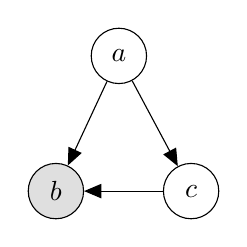
\begin{tikzpicture}
      % Define nodes
      \node[latent, obs]             (b) {$b$};
      \node[latent, above=of b, xshift=0.8cm] (a) {$a$};
      \node[latent, right=of b]       (c) {$c$};
      % Connect nodes
      \edge {a} {b};
      \edge {a} {c};
      \edge {c} {b};
    \end{tikzpicture} \\
    Cascade from a to c. V-structure from b to a and c.
\end{subfigure}
\end{figure}


\clearpage 

\paragraph{Factor Graph (b) to BN}
Converting to Bayesian Networks while maintaining conditional independence in \ref{equation:conditionalIndependenceB} has two different solutions. 

Solution 1:
\begin{figure}[!htb]
\centering
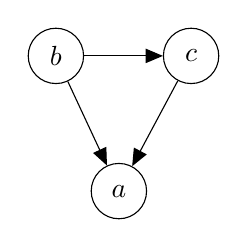
\begin{tikzpicture}
  % Define nodes
  \node[latent]             (a) {$a$};
  \node[latent, above=of a, xshift=-0.8cm] (b) {$b$};
  \node[latent, right=of b]       (c) {$c$};
  % Connect nodes
  \edge {b} {a};
  \edge {c} {a};
  \edge {b} {c};
\end{tikzpicture}
\end{figure}
%
\begin{equation}
\label{equation:conditionalIndependenceBNbSolution1}
\begin{split}
P(a,b,c) = P(a|b,c)P(c|b)P(b) = \frac{1}{Z} f_{1}(b)f_{2}(c)f_{3}(a,b)f_{4}(a,c)f_{5}(b,c) \\
Z = \sum_{a,b,c} f_{1}(b)f_{2}(c)f_{3}(a,b)f_{4}(a,c)f_{5}(b,c) \\
\end{split}
\end{equation}
%
\begin{figure}[!htb]
\centering
\begin{subfigure}[t]{0.3\textwidth}
	\centering
    \caption*{$b \nci c | a$}
    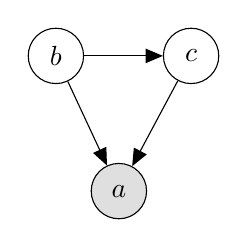
\begin{tikzpicture}
      % Define nodes
      \node[latent, obs]             (a) {$a$};
      \node[latent, above=of a, xshift=-0.8cm] (b) {$b$};
      \node[latent, right=of b]       (c) {$c$};
      % Connect nodes
      \edge {b} {a};
      \edge {c} {a};
      \edge {b} {c};
    \end{tikzpicture} \\
	Cascade from b to c, V-structure from a to b and c
\end{subfigure}
\begin{subfigure}[t]{0.3\textwidth}
	\centering
    \caption*{$a \nci b | c$}
	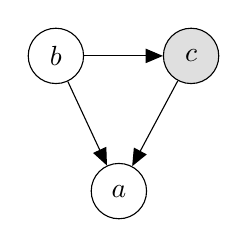
\begin{tikzpicture}
      % Define nodes
      \node[latent]             (a) {$a$};
      \node[latent, above=of a, xshift=-0.8cm] (b) {$b$};
      \node[latent, obs, right=of b]       (c) {$c$};
      % Connect nodes
      \edge {b} {a};
      \edge {c} {a};
      \edge {b} {c};
    \end{tikzpicture} \\
    Cascade from b to a
\end{subfigure}
\begin{subfigure}[t]{0.3\textwidth}
	\centering
    \caption*{$a \nci c | b$}
    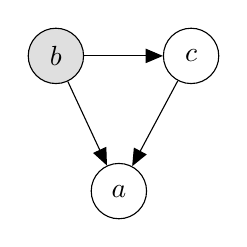
\begin{tikzpicture}
      % Define nodes
      \node[latent]             (a) {$a$};
      \node[latent, obs, above=of a, xshift=-0.8cm] (b) {$b$};
      \node[latent, right=of b]       (c) {$c$};
      % Connect nodes
      \edge {b} {a};
      \edge {c} {a};
      \edge {b} {c};
    \end{tikzpicture} \\
    Cascade from c to a
\end{subfigure}
\end{figure}

\clearpage

Solution 2:
\begin{figure}[!htb]
\centering
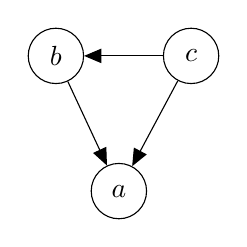
\begin{tikzpicture}
  % Define nodes
  \node[latent]             (a) {$a$};
  \node[latent, above=of a, xshift=-0.8cm] (b) {$b$};
  \node[latent, right=of b]       (c) {$c$};
  % Connect nodes
  \edge {b} {a};
  \edge {c} {a};
  \edge {c} {b};
\end{tikzpicture}
\end{figure}
%
\begin{equation}
\label{equation:conditionalIndependenceBNbSolution2}
\begin{split}
P(a,b,c) = P(a|b,c)P(b|c)P(c)  = \frac{1}{Z} f_{1}(b)f_{2}(c)f_{3}(a,b)f_{4}(a,c)f_{5}(b,c) \\
Z = \sum_{a,b,c} f_{1}(b)f_{2}(c)f_{3}(a,b)f_{4}(a,c)f_{5}(b,c) \\
\end{split}
\end{equation}
%
\begin{figure}[!htb]
\centering
\begin{subfigure}[t]{0.3\textwidth}
	\centering
    \caption*{$b \nci c | a$}
    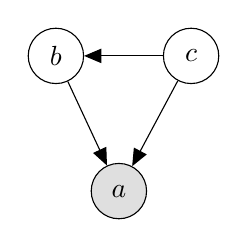
\begin{tikzpicture}
      % Define nodes
      \node[latent, obs]             (a) {$a$};
      \node[latent, above=of a, xshift=-0.8cm] (b) {$b$};
      \node[latent, right=of b]       (c) {$c$};
      % Connect nodes
      \edge {b} {a};
      \edge {c} {a};
      \edge {c} {b};
    \end{tikzpicture} \\
    Cascade from c to b, V-structure from a to b and c
\end{subfigure}
\begin{subfigure}[t]{0.3\textwidth}
	\centering
    \caption*{$a \nci b | c$}
    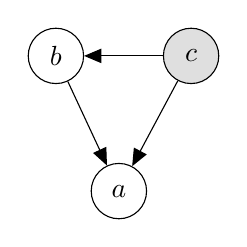
\begin{tikzpicture}
      % Define nodes
      \node[latent]             (a) {$a$};
      \node[latent, above=of a, xshift=-0.8cm] (b) {$b$};
      \node[latent, obs, right=of b]       (c) {$c$};
      % Connect nodes
      \edge {b} {a};
      \edge {c} {a};
      \edge {c} {b};
    \end{tikzpicture} \\
    Cascade from b to a 
\end{subfigure}
\begin{subfigure}[t]{0.3\textwidth}
	\centering
    \caption*{$a \nci c | b$}
    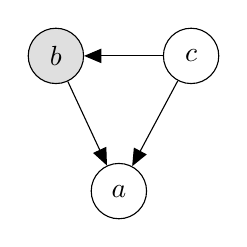
\begin{tikzpicture}
      % Define nodes
      \node[latent]             (a) {$a$};
      \node[latent, obs, above=of a, xshift=-0.8cm] (b) {$b$};
      \node[latent, right=of b]       (c) {$c$};
      % Connect nodes
      \edge {b} {a};
      \edge {c} {a};
      \edge {c} {b};
    \end{tikzpicture} \\
    Cascade from c to a
\end{subfigure}
\end{figure}

\clearpage

%------------------------------------------------------------------
\subsubsubsection{Factor Graph to MRF}

\paragraph{Factor Graph (a) to MRF}
Converting to Markov Random Field while maintaining conditional independence in \ref{equation:conditionalIndependenceA}.

\begin{figure}[!htb]
\centering
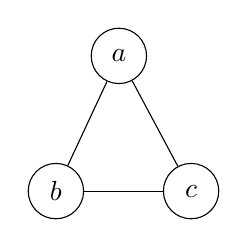
\begin{tikzpicture}
  % Define nodes
  \node[latent]             (b) {$b$};
  \node[latent, above=of b, xshift=0.8cm] (a) {$a$};
  \node[latent, right=of b]       (c) {$c$};
  % Connect nodes
  \edge[-] {a} {b};
  \edge[-] {a} {c};
  \edge[-] {c} {b};
\end{tikzpicture}
\end{figure}
%
\begin{equation}
\label{equation:conditionalIndependenceMRFaSolution}
\psi_{1}(a,b,c) = f_{1}(a,b,c)f_{2}(a)
\end{equation}
%
\begin{figure}[!htb]
\centering
\begin{subfigure}[t]{0.3\textwidth}
	\centering	
    \caption*{$b \nci c | a$}
    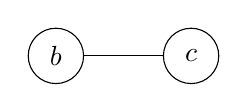
\begin{tikzpicture}
  % Define nodes
  \node[latent]             (b) {$b$};
  \node[latent, right=of b]       (c) {$c$};
  % Connect nodes
  \edge[-] {c} {b};
\end{tikzpicture}
\end{subfigure}
\begin{subfigure}[t]{0.3\textwidth}
	\centering	
    \caption*{$a \nci b | c$}
    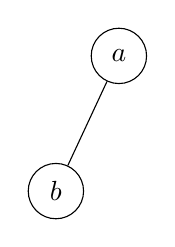
\begin{tikzpicture}
  % Define nodes
  \node[latent]             (b) {$b$};
  \node[latent, above=of b, xshift=0.8cm] (a) {$a$};
  % Connect nodes
  \edge[-] {a} {b};
\end{tikzpicture}
\end{subfigure}
\begin{subfigure}[t]{0.3\textwidth}
	\centering	
    \caption*{$a \nci c | b$}
    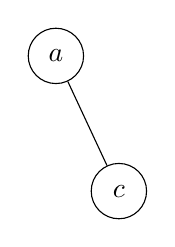
\begin{tikzpicture}
  % Define nodes
  \node[latent] (a) {$a$};
  \node[latent, below=of a, xshift=0.8cm]       (c) {$c$};
  % Connect nodes
  \edge[-] {a} {c};
\end{tikzpicture}
\end{subfigure}
\end{figure}
\clearpage
\paragraph{Factor Graph (b) to MRF}
Converting to Markov Random Field while maintaining conditional independence in \ref{equation:conditionalIndependenceB}.
%
\begin{figure}[!htb]
\centering
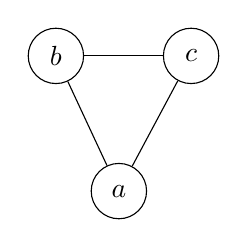
\begin{tikzpicture}
  % Define nodes
  % Define nodes
  \node[latent]             (a) {$a$};
  \node[latent, above=of a, xshift=-0.8cm] (b) {$b$};
  \node[latent, right=of b]       (c) {$c$};
  % Connect nodes
  \edge[-] {b} {a};
  \edge[-] {c} {a};
  \edge[-] {c} {b};
  % Connect the nodes
\end{tikzpicture}
\end{figure}
%
\begin{equation}
\label{equation:conditionalIndependenceMRFbSolution}
\psi_{1}(a,b,c) = f_{1}(b)f_{2}(c)f_{3}(a,b)f_{4}(a,c)f_{5}(b,c)
\end{equation}
%
\begin{figure}[!htb]
\centering
\begin{subfigure}[t]{0.3\textwidth}
	\centering	
    \caption*{$b \nci c | a$}
    \begin{tikzpicture}
  % Define nodes
  % Define nodes
  \node[latent, above=of a, xshift=-0.8cm] (b) {$b$};
  \node[latent, right=of b]       (c) {$c$};
  % Connect nodes
  \edge[-] {c} {b};
  % Connect the nodes
\end{tikzpicture}
\end{subfigure}
\begin{subfigure}[t]{0.3\textwidth}
	\centering	
    \caption*{$a \nci b | c$}
    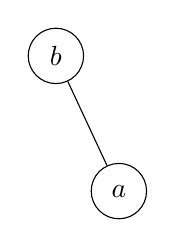
\begin{tikzpicture}
  % Define nodes
  % Define nodes
  \node[latent]             (a) {$a$};
  \node[latent, above=of a, xshift=-0.8cm] (b) {$b$};
  % Connect nodes
  \edge[-] {b} {a};
  % Connect the nodes
\end{tikzpicture}
\end{subfigure}
\begin{subfigure}[t]{0.3\textwidth}
	\centering	
    \caption*{$a \nci c | b$}
    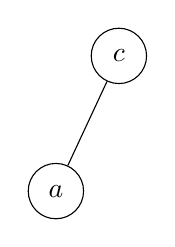
\begin{tikzpicture}
  % Define nodes
  % Define nodes
  \node[latent]             (a) {$a$};
  \node[latent, above=of a, xshift=0.8cm]       (c) {$c$};
  % Connect nodes
  \edge[-] {c} {a};
  % Connect the nodes
\end{tikzpicture}
\end{subfigure}
\end{figure}

\clearpage

%------------------------------------------------------------------
\subsubsection{Markov Random Field}
\begin{figure}[!htb]
\centering
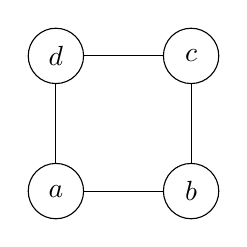
\begin{tikzpicture}
  % Define nodes
  \node[latent]       (a) {$a$};
  \node[latent, right=of a] (b) {$b$};
  \node[latent, above=of b] (c) {$c$};
  \node[latent, above=of a] (d) {$d$};
  \edge[-] {a} {b,d} ;
  \edge[-] {c} {b,d} ;
\end{tikzpicture}
\end{figure}

The conditional independence properties for Markov Random Field are
shown in equations \ref{equation:conditionalIndependenceMRFSingle} (conditioned upon 1 variable) and \ref{equation:conditionalIndependenceMRFPair} (conditioned upon 2 variables). Equation \ref{equation:conditionalIndependenceMRFNone} shows the marginal independence properties. However, we have assumed in this questions that the marginal independence properties do not have to be maintained. Instead, we seek for generality by showing we can convert to Factor Graph while maintaining the marginal independences in  \ref{equation:conditionalIndependenceMRFNone} whereas we show we cannot convert to Bayesian Networks regardless of whether or not we maintain marginal independence properties in \ref{equation:conditionalIndependenceMRFNone}.

\begin{equation}
\label{equation:conditionalIndependenceMRFNone}
\begin{split}
a \nci b | \emptyset = a \nci b \\
a \nci c | \emptyset = a \nci c \\
a \nci d | \emptyset = a \nci d \\
b \nci c | \emptyset = b \nci c \\
b \nci d | \emptyset = b \nci d \\
c \nci d | \emptyset = c \nci d  
\end{split}
\end{equation}

\clearpage 

\begin{equation}
\label{equation:conditionalIndependenceMRFSingle}
\begin{split}
b \nci c | a \\
b \nci d | a \\
c \nci d | a \\
a \nci c | b \\
a \nci d | b \\
c \nci d | b \\
a \nci b | c \\
a \nci d | c \\
b\nci d | c \\
a \nci b | d \\
a \nci c | d \\
b \nci c | d 
\end{split}
\end{equation}

\begin{figure}[!htb]
\centering
\begin{subfigure}[t]{0.45\textwidth}
	\centering	
    \caption*{$b \nci c | a $ and
		$b \nci d | a $ and
		$c \nci d | a $}
    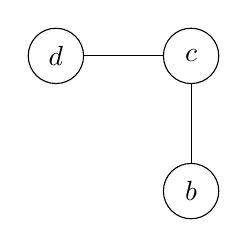
\begin{tikzpicture}
      % Define nodes
      \node[latent] (b) {$b$};
      \node[latent, above=of b] (c) {$c$};
      \node[latent, left=of c] (d) {$d$};
      \edge[-] {c} {b,d} ;
    \end{tikzpicture}
\end{subfigure}
\begin{subfigure}[t]{0.45\textwidth}
	\centering	
    \caption*{$a \nci c | b$ and
        $a \nci d | b$ and
        $c \nci d | b$}
    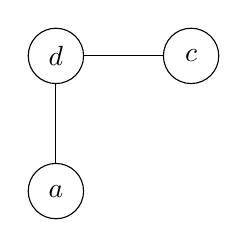
\begin{tikzpicture}
      % Define nodes
      \node[latent]       (a) {$a$};
      \node[latent, above=of a] (d) {$d$};
      \node[latent, right=of d] (c) {$c$};
      \edge[-] {d} {a,c} ;
    \end{tikzpicture}
\end{subfigure}
\\ \vspace{2em}
\begin{subfigure}[t]{0.45\textwidth}
	\centering	
    \caption*{$a \nci b | c$ and
          $a \nci d | c$ and
          $b \nci d | c$}
    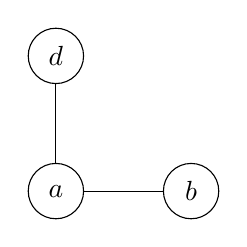
\begin{tikzpicture}
      % Define nodes
      \node[latent]       (a) {$a$};
      \node[latent, right=of a] (b) {$b$};
      \node[latent, above=of a] (d) {$d$};
      \edge[-] {a} {b,d} ;
    \end{tikzpicture}
\end{subfigure}
\begin{subfigure}[t]{0.45\textwidth}
	\centering	
    \caption*{$a \nci b | d$ and
          $a \nci c | d$ and
          $b \nci c | d$}
    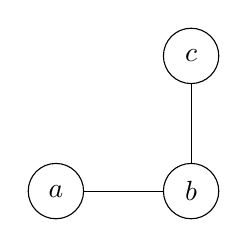
\begin{tikzpicture}
      % Define nodes
      \node[latent]       (a) {$a$};
      \node[latent, right=of a] (b) {$b$};
      \node[latent, above=of b] (c) {$c$};
      \edge[-] {b} {a,c} ;
    \end{tikzpicture}
\end{subfigure}
\end{figure}
\clearpage 
%
\begin{equation}
\label{equation:conditionalIndependenceMRFPair}
\begin{split}
a \ci c | b, d \\
b \ci d | a, c \\
b \nci a | c, d \\
b \nci c | a, d \\
c \nci d | a, b \\
a \nci d | b, c
\end{split}
\end{equation}

\begin{figure}[!htb]
\centering
\begin{subfigure}[t]{0.3\textwidth}
	\centering	
    \caption*{$a \ci c | b, d$}
    \begin{tikzpicture}
      % Define nodes
      \node[latent]       (a) {$a$};
      \node[latent, above=of a, xshift=2.0cm] (c) {$c$};
    \end{tikzpicture}
\end{subfigure}
\begin{subfigure}[t]{0.3\textwidth}
	\centering	
    \caption*{$b \ci d | a, c$}
    \begin{tikzpicture}
      % Define nodes
      \node[latent] (b) {$b$};
      \node[latent, above=of b, xshift=-2.0cm] (d) {$d$};
    \end{tikzpicture}
\end{subfigure}
\begin{subfigure}[t]{0.3\textwidth}
	\centering	
    \caption*{$b \nci a | c, d$}
    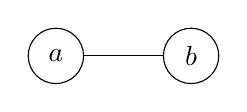
\begin{tikzpicture}
      % Define nodes
      \node[latent]       (a) {$a$};
      \node[latent, right=of a] (b) {$b$};
      \edge[-] {a} {b} ;
    \end{tikzpicture}
\end{subfigure}
\\ \vspace{2em}
\begin{subfigure}[t]{0.3\textwidth}
	\centering	
    \caption*{$b \nci c | a, d$}
    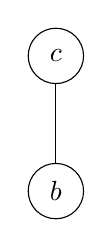
\begin{tikzpicture}
      % Define nodes
      \node[latent] (b) {$b$};
      \node[latent, above=of b] (c) {$c$};
      \edge[-] {c} {b} ;
    \end{tikzpicture}
\end{subfigure}
\begin{subfigure}[t]{0.3\textwidth}
	\centering	
    \caption*{$c \nci d | a, b$}
    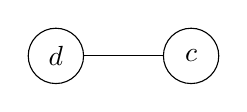
\begin{tikzpicture}
      % Define nodes
      \node[latent] (c) {$c$};
      \node[latent, left=of c] (d) {$d$};
      \edge[-] {c} {d} ;
    \end{tikzpicture}
\end{subfigure}
\begin{subfigure}[t]{0.3\textwidth}
	\centering	
    \caption*{$a \nci d | b, c$}
    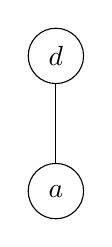
\begin{tikzpicture}
      % Define nodes
      \node[latent]       (a) {$a$};
      \node[latent, above=of a] (d) {$d$};
      \edge[-] {a} {d} ;
    \end{tikzpicture}
\end{subfigure}
\end{figure}
\clearpage 
%------------------------------------------------------------------
\subsubsubsection{MRF to Factor Graph}
\begin{figure}[!htb]
\centering
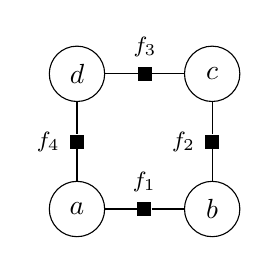
\begin{tikzpicture}
  % Define nodes
  \node[latent]       (a) {$a$};
  \node[latent, right=of a] (b) {$b$};
  \node[latent, above=of b] (c) {$c$};
  \node[latent, above=of a] (d) {$d$};
  \factor[right=of a] {factor1} {$f_1$} {} {};
  \factor[above=of b] {factor2} {left:$f_2$} {} {};
  \factor[left=of c] {factor3} {$f_3$} {} {};
  \factor[above=of a] {factor4} {left:$f_4$} {} {};
  \factoredge[-] {a} {factor1} {b};
  \factoredge[-] {b} {factor2} {c};
  \factoredge[-] {c} {factor3} {d};
  \factoredge[-] {d} {factor4} {a};
\end{tikzpicture}
\end{figure}

The proof for conditional independence have a similar looking graph as the Markov Random Field itself. Also, according to slide 9 of Lecture 18 ECE521 Winter 2017, it is shown that Markov Random Field is a subset of Factor Graph, meaning that all Markov Random Field can be represented by Factor Graphs. This means that it must always be possible to convert any Markov Random Field to a Factor Graph. 

\begin{figure}[!htb]
\centering
\begin{subfigure}[t]{0.48\textwidth}
	\centering	
    \caption*{$a \ci c | b, d$}
    \begin{tikzpicture}
      % Define nodes
      \node[latent]       (a) {$a$};
      \node[latent, above=of a, xshift=2.0cm] (c) {$c$};
    \end{tikzpicture}
\end{subfigure}
\begin{subfigure}[t]{0.48\textwidth}
	\centering	
    \caption*{$b \ci d | a, c$}
    \begin{tikzpicture}
      % Define nodes
      \node[latent] (b) {$b$};
      \node[latent, above=of b, xshift=-2.0cm] (d) {$d$};
    \end{tikzpicture}
\end{subfigure}
\end{figure}

\clearpage 
%------------------------------------------------------------------
\subsubsubsection{MRF to BN}
Conversion from Markov Random Field (MRF) above to Bayesian Networks (BN) does not exist. Bayesian Networks are acyclic directed graphs. 

Therefore, below are the all possible factorizations of the MRF to BN which are acyclic and follows the conversion rule given in lectures (every edge that exist in MRF must also exist in the BN to be able to convert it back into an equivalent MRF), each with a different possible acyclic pair of root to leaf paths of the BN.

Since there must be an edge, each edge can be in 1 of 2 directions. There are 4 edges, so there are $2^{4} = 16$ possible factorizations. 2 of the factorizations results in directed cycles, which is not a BN by definition. Below we show the remaining $14$ ($16 - 2 = 14$) acyclic possible factorizations. 

\begin{figure}[!htb]
\centering
\begin{subfigure}[t]{0.48\textwidth}
	\centering	
    \caption*{Root a, Leaf c}
    \begin{tikzpicture}
      % Define nodes
      \node[latent]       (a) {$a$};
      \node[latent, right=of a] (b) {$b$};
      \node[latent, above=of b] (c) {$c$};
      \node[latent, above=of a] (d) {$d$};
      \edge {a} {b,d} ;
      \edge {b,d} {c} ;
    \end{tikzpicture}
\end{subfigure}
\begin{subfigure}[t]{0.48\textwidth}
	\centering	
    \caption*{Root c, Leaf a}
    \begin{tikzpicture}
      % Define nodes
      \node[latent]       (a) {$a$};
      \node[latent, right=of a] (b) {$b$};
      \node[latent, above=of b] (c) {$c$};
      \node[latent, above=of a] (d) {$d$};
      \edge {c} {b,d} ;
      \edge {b,d} {a} ;
    \end{tikzpicture}
\end{subfigure}
\\ \vspace{2em}
\begin{subfigure}[t]{0.48\textwidth}
	\centering	
    \caption*{Root b, Leaf d}
    \begin{tikzpicture}
      % Define nodes
      \node[latent]       (a) {$a$};
      \node[latent, right=of a] (b) {$b$};
      \node[latent, above=of b] (c) {$c$};
      \node[latent, above=of a] (d) {$d$};
      \edge {b} {a,c} ;
      \edge {a,c} {d} ;
    \end{tikzpicture}
\end{subfigure}
\begin{subfigure}[t]{0.48\textwidth}
	\centering	
    \caption*{Root d, Leaf b}
    \begin{tikzpicture}
      % Define nodes
      \node[latent]       (a) {$a$};
      \node[latent, right=of a] (b) {$b$};
      \node[latent, above=of b] (c) {$c$};
      \node[latent, above=of a] (d) {$d$};
      \edge {d} {a,c} ;
      \edge {a,c} {b} ;
    \end{tikzpicture}
\end{subfigure}
% New stuff
\begin{subfigure}[t]{0.48\textwidth}
	\centering	
    \caption*{Root a, Leaf b}
    \begin{tikzpicture}
      % Define nodes
      \node[latent]       (a) {$a$};
      \node[latent, right=of a] (b) {$b$};
      \node[latent, above=of b] (c) {$c$};
      \node[latent, above=of a] (d) {$d$};
      \edge {a} {b,d} ;
      \edge {d} {c} ;
      \edge {c} {b} ;
    \end{tikzpicture}
\end{subfigure}
\begin{subfigure}[t]{0.48\textwidth}
	\centering	
    \caption*{Root a, Leaf d}
    \begin{tikzpicture}
      % Define nodes
      \node[latent]       (a) {$a$};
      \node[latent, right=of a] (b) {$b$};
      \node[latent, above=of b] (c) {$c$};
      \node[latent, above=of a] (d) {$d$};
      \edge {a} {b,d} ;
      \edge {b} {c} ;
      \edge {c} {d} ;
    \end{tikzpicture}
\end{subfigure}
\begin{subfigure}[t]{0.48\textwidth}
	\centering	
    \caption*{Root b, Leaf a}
    \begin{tikzpicture}
      % Define nodes
      \node[latent]       (a) {$a$};
      \node[latent, right=of a] (b) {$b$};
      \node[latent, above=of b] (c) {$c$};
      \node[latent, above=of a] (d) {$d$};
      \edge {b} {a,c} ;
      \edge {c} {d} ;
      \edge {d} {a} ;
    \end{tikzpicture}
\end{subfigure}
\begin{subfigure}[t]{0.48\textwidth}
	\centering	
    \caption*{Root b, Leaf c}
    \begin{tikzpicture}
      % Define nodes
      \node[latent]       (a) {$a$};
      \node[latent, right=of a] (b) {$b$};
      \node[latent, above=of b] (c) {$c$};
      \node[latent, above=of a] (d) {$d$};
      \edge {b} {a,c} ;
      \edge {a} {d} ;
      \edge {d} {c} ;
    \end{tikzpicture}
\end{subfigure}
\begin{subfigure}[t]{0.48\textwidth}
	\centering	
    \caption*{Root c, Leaf b}
    \begin{tikzpicture}
      % Define nodes
      \node[latent]       (a) {$a$};
      \node[latent, right=of a] (b) {$b$};
      \node[latent, above=of b] (c) {$c$};
      \node[latent, above=of a] (d) {$d$};
      \edge {c} {b,d} ;
      \edge {d} {a} ;
      \edge {a} {b} ;
    \end{tikzpicture}
\end{subfigure}
\begin{subfigure}[t]{0.48\textwidth}
	\centering	
    \caption*{Root c, Leaf d}
    \begin{tikzpicture}
      % Define nodes
      \node[latent]       (a) {$a$};
      \node[latent, right=of a] (b) {$b$};
      \node[latent, above=of b] (c) {$c$};
      \node[latent, above=of a] (d) {$d$};
      \edge {c} {b,d} ;
      \edge {b} {a} ;
      \edge {a} {d} ;
    \end{tikzpicture}
\end{subfigure}
\begin{subfigure}[t]{0.48\textwidth}
	\centering	
    \caption*{Root d, Leaf a}
    \begin{tikzpicture}
      % Define nodes
      \node[latent]       (a) {$a$};
      \node[latent, right=of a] (b) {$b$};
      \node[latent, above=of b] (c) {$c$};
      \node[latent, above=of a] (d) {$d$};
      \edge {d} {a,c} ;
      \edge {c} {b} ;
      \edge {b} {a} ;
    \end{tikzpicture}
\end{subfigure}
\begin{subfigure}[t]{0.48\textwidth}
	\centering	
    \caption*{Root d, Leaf c}
    \begin{tikzpicture}
      % Define nodes
      \node[latent]       (a) {$a$};
      \node[latent, right=of a] (b) {$b$};
      \node[latent, above=of b] (c) {$c$};
      \node[latent, above=of a] (d) {$d$};
      \edge {d} {a,c} ;
      \edge {a} {b} ;
      \edge {b} {c} ;
    \end{tikzpicture}
\end{subfigure}
\begin{subfigure}[t]{0.48\textwidth}
	\centering	
    \caption*{Root b and d, Leaf a and c}
    \begin{tikzpicture}
      % Define nodes
      \node[latent]       (a) {$a$};
      \node[latent, right=of a] (b) {$b$};
      \node[latent, above=of b] (c) {$c$};
      \node[latent, above=of a] (d) {$d$};
      \edge {d} {a,c} ;
      \edge {b} {a, c} ;
    \end{tikzpicture}
\end{subfigure}
\begin{subfigure}[t]{0.48\textwidth}
	\centering	
    \caption*{Root a and c, Leaf b and d}
    \begin{tikzpicture}
      % Define nodes
      \node[latent]       (a) {$a$};
      \node[latent, right=of a] (b) {$b$};
      \node[latent, above=of b] (c) {$c$};
      \node[latent, above=of a] (d) {$d$};
      \edge {c} {b, d} ;
      \edge {a} {b, d} ;
    \end{tikzpicture}
\end{subfigure}
\end{figure}

\clearpage

We can Proof by Counter Example that each of the possible factorization above does not satisfy at least one of the conditional independence properties given in equation \ref{equation:conditionalIndependenceMRFPair}.

Root a, Leaf c:
\begin{tikzpicture}
  % Define nodes
  \node[latent, obs]       (a) {$a$};
  \node[latent, right=of a] (b) {$b$};
  \node[latent, obs, above=of b] (c) {$c$};
  \node[latent, above=of a] (d) {$d$};
  \edge {a} {b,d} ;
  \edge {b,d} {c} ;
\end{tikzpicture}
but $b \nci d | a,c$  due to V-structure from c to b and d.

Root c, Leaf a:
\begin{tikzpicture}
  % Define nodes
  \node[latent, obs]       (a) {$a$};
  \node[latent, right=of a] (b) {$b$};
  \node[latent, obs, above=of b] (c) {$c$};
  \node[latent, above=of a] (d) {$d$};
  \edge {c} {b,d} ;
  \edge {b,d} {a} ;
\end{tikzpicture}
but $b \nci d | a,c$ due to V-structure from a to b and d.

Root b, Leaf d:
\begin{tikzpicture}
  % Define nodes
  \node[latent]       (a) {$a$};
  \node[latent, obs, right=of a] (b) {$b$};
  \node[latent, above=of b] (c) {$c$};
  \node[latent, obs, above=of a] (d) {$d$};
  \edge {b} {a,c} ;
  \edge {a,c} {d} ;
\end{tikzpicture}
but $a \nci c| b,d$ due to V-structure from d to a and c.

Root d, Leaf b:
\begin{tikzpicture}
  % Define nodes
  \node[latent]       (a) {$a$};
  \node[latent, obs, right=of a] (b) {$b$};
  \node[latent, above=of b] (c) {$c$};
  \node[latent, obs, above=of a] (d) {$d$};
  \edge {d} {a,c} ;
  \edge {a,c} {b} ;
\end{tikzpicture}
but $a \nci c| b,d$ due to V-structure from b to a and c.

% New stuff
Root a, Leaf b:
\begin{tikzpicture}
% Define nodes
\node[latent]       (a) {$a$};
\node[latent, obs, right=of a] (b) {$b$};
\node[latent, above=of b] (c) {$c$};
\node[latent, obs, above=of a] (d) {$d$};
\edge {a} {b,d} ;
\edge {d} {c} ;
\edge {c} {b} ;
\end{tikzpicture}
but $a \nci c| b,d$ due to V-structure from b to a and c.

Root a, Leaf d:
\begin{tikzpicture}
% Define nodes
\node[latent]       (a) {$a$};
\node[latent, obs, right=of a] (b) {$b$};
\node[latent, above=of b] (c) {$c$};
\node[latent, obs, above=of a] (d) {$d$};
\edge {a} {b,d} ;
\edge {b} {c} ;
\edge {c} {d} ;
\end{tikzpicture}
but $a \nci c| b,d$ due to V-structure from d to a and c.

Root b, Leaf a:
\begin{tikzpicture}
% Define nodes
\node[latent, obs]       (a) {$a$};
\node[latent, right=of a] (b) {$b$};
\node[latent, obs, above=of b] (c) {$c$};
\node[latent, above=of a] (d) {$d$};
\edge {b} {a,c} ;
\edge {c} {d} ;
\edge {d} {a} ;
\end{tikzpicture}
but $b \nci d | a,c$ due to V-structure from a to b and d.

Root b, Leaf c:
\begin{tikzpicture}
% Define nodes
\node[latent, obs]       (a) {$a$};
\node[latent, right=of a] (b) {$b$};
\node[latent, obs, above=of b] (c) {$c$};
\node[latent, above=of a] (d) {$d$};
\edge {b} {a,c} ;
\edge {a} {d} ;
\edge {d} {c} ;
\end{tikzpicture}
but $b \nci d | a,c$ due to V-structure from c to b and d.

Root c, Leaf b:
\begin{tikzpicture}
% Define nodes
\node[latent]       (a) {$a$};
\node[latent, obs, right=of a] (b) {$b$};
\node[latent, above=of b] (c) {$c$};
\node[latent, obs, above=of a] (d) {$d$};
\edge {c} {b,d} ;
\edge {d} {a} ;
\edge {a} {b} ;
\end{tikzpicture}
but $a \nci c| b,d$ due to V-structure from b to a and c.

Root c, Leaf d:
\begin{tikzpicture}
% Define nodes
\node[latent]       (a) {$a$};
\node[latent, obs, right=of a] (b) {$b$};
\node[latent, above=of b] (c) {$c$};
\node[latent, obs, above=of a] (d) {$d$};
\edge {c} {b,d} ;
\edge {b} {a} ;
\edge {a} {d} ;
\end{tikzpicture}
but $a \nci c| b,d$ due to V-structure from d to a and c.


Root d, Leaf a:
\begin{tikzpicture}
% Define nodes
\node[latent, obs]       (a) {$a$};
\node[latent, right=of a] (b) {$b$};
\node[latent, obs, above=of b] (c) {$c$};
\node[latent, above=of a] (d) {$d$};
\edge {d} {a,c} ;
\edge {c} {b} ;
\edge {b} {a} ;
\end{tikzpicture}
but $b \nci d | a,c$ due to V-structure from a to b and d.

Root d, Leaf c:
\begin{tikzpicture}
% Define nodes
\node[latent, obs]       (a) {$a$};
\node[latent, right=of a] (b) {$b$};
\node[latent, obs, above=of b] (c) {$c$};
\node[latent, above=of a] (d) {$d$};
\edge {d} {a,c} ;
\edge {a} {b} ;
\edge {b} {c} ;
\end{tikzpicture}
but $b \nci d | a,c$ due to V-structure from c to b and d.

Root b and d, Leaf a and c:
\begin{tikzpicture}
% Define nodes
\node[latent, obs]       (a) {$a$};
\node[latent, right=of a] (b) {$b$};
\node[latent, obs, above=of b] (c) {$c$};
\node[latent, above=of a] (d) {$d$};
\edge {d} {a,c} ;
\edge {b} {a, c} ;
\end{tikzpicture}
but $b \nci d | a,c $ due to V-structure from a and c to b and d.

Root a and c, Leaf b and d:
\begin{tikzpicture}
% Define nodes
\node[latent]       (a) {$a$};
\node[latent, obs, right=of a] (b) {$b$};
\node[latent, above=of b] (c) {$c$};
\node[latent, obs, above=of a] (d) {$d$};
\edge {c} {b, d} ;
\edge {a} {b, d} ;
\end{tikzpicture}
but $a \nci c | b,d $ due to V-structure from b and d to a and c.


Thus, we have explained that there is no equivalent Bayesian Networks that implies the same conditional independence properties as the Markov Random Field. 

This can be concisely explained and proven below. 

To satisfy $a \nci c | d$ in equation \ref{equation:conditionalIndependenceMRFSingle}, 
there needs to be a path from $a$ to $c$ (path from $c$ to $a$ would just be a symmetric argument). The path must go through $b$. 

\begin{tikzpicture}
% Define nodes
\node[latent]       (a) {$a$};
\node[latent, right=of a] (b) {$b$};
\node[latent, above=of b] (c) {$c$};
\node[latent, obs, above=of a] (d) {$d$};
\edge {a} {b} ;
\edge {b} {c} ;
\end{tikzpicture}

Now, in order to satisfy $b \nci d | a$ in equation \ref{equation:conditionalIndependenceMRFSingle}, 
there needs to be a path from $b$ to $d$. (Path from $d$ to $b$ would just be a symmetric argument). The only possible path is through $c$. 

\begin{tikzpicture}
% Define nodes
\node[latent, obs]       (a) {$a$};
\node[latent, right=of a] (b) {$b$};
\node[latent, above=of b] (c) {$c$};
\node[latent, above=of a] (d) {$d$};
\edge {b} {c} ;
\edge {c} {d} ;
\end{tikzpicture}

Combining both, we get. 

\begin{tikzpicture}
% Define nodes
\node[latent]       (a) {$a$};
\node[latent, right=of a] (b) {$b$};
\node[latent, above=of b] (c) {$c$};
\node[latent, above=of a] (d) {$d$};
\edge {a} {b} ;
\edge {b} {c} ;
\edge {c} {d} ;
\end{tikzpicture}

This currently does not satisfy $a \nci d |b, c$ in equation \ref{equation:conditionalIndependenceMRFPair}. Therefore, we need to try adding an edge between $a$ and $d$. The only possible assignment is from $a$ to $d$ as 
$d$ to $a$ results in an acyclic directed graph which is not a Bayesian Network by definition. 
Our final factorization results in 

\begin{tikzpicture}
% Define nodes
\node[latent]       (a) {$a$};
\node[latent, right=of a] (b) {$b$};
\node[latent, above=of b] (c) {$c$};
\node[latent, above=of a] (d) {$d$};
\edge {a} {b,d} ;
\edge {b} {c} ;
\edge {c} {d} ;
\end{tikzpicture}

However, this does not satisfy $a \ci c | b, d$ as shown below due to V-structure from d to a and c. 

\begin{tikzpicture}
% Define nodes
\node[latent]       (a) {$a$};
\node[latent, obs, right=of a] (b) {$b$};
\node[latent, above=of b] (c) {$c$};
\node[latent, obs, above=of a] (d) {$d$};
\edge {a} {b,d} ;
\edge {b} {c} ;
\edge {c} {d} ;
\end{tikzpicture}

Therefore, there is no possible BN factorization for the given MRF as we have shown it is impossible to satisfy all the conditional independence properties. 

\clearpage
%------------------------------------------------------------------
\subsection{Conditional Independence in Bayesian Networks}
\begin{figure}
\centering
\begin{tikzpicture}
  % Define nodes
  \node[latent]             (c) {$c$};
  \node[latent, above=of c] (e) {$e$};
  \node[latent, right=of e] (b) {$b$};
  \node[latent, above=of b] (a) {$a$};
  \node[latent, right=of c] (d) {$d$};
  \node[latent, right=of d] (f) {$f$};
  % Connect the nodes
  \edge {b,e} {c};
  \edge {a} {b};
  \edge {b,c} {d};
  \edge {b} {f};
\end{tikzpicture}
\end{figure}

\subsubsection{Express Joint Probability of Bayesian Networks}
\begin{equation}
\label{equation:JointProbBN}
P(a,b,c,d,e,f) = P(d|b,c)P(c|b,e)P(e)P(f|b)P(b|a)P(a)
\end{equation}

\subsubsection{Determine TRUE or FALSE}
\subsubsubsection{$a \ci c$}
FALSE

Cascade from a to b to c. \hspace{2em}
\begin{tikzpicture}
  % Define nodes
  \node[latent]             (a) {$a$};
  \node[latent, below=of a] (b) {$b$};
  \node[latent, below=of b, xshift=-0.8cm] (c) {$c$};
  % Connect the nodes
  \edge {a} {b};
  \edge {b} {c};
\end{tikzpicture}

This shows that $a \nci c$. 

\clearpage
\subsubsubsection{$a \ci c \given b$}
TRUE

Cascade from a to c is blocked given b. \hspace{2em}
\begin{tikzpicture}
  % Define nodes
  \node[latent]             (a) {$a$};
  \node[latent, obs, below=of a] (b) {$b$};
  \node[latent, below=of b, xshift=-0.8cm] (c) {$c$};
  % Connect the nodes
  \edge {a} {b};
  \edge {b} {c};
\end{tikzpicture}

This shows that $a \ci c \given b$. 

\subsubsubsection{$e \ci b$}
TRUE

V-structure from b and e to c are blocked if c is not given. \hspace{2em}
\begin{tikzpicture}
  % Define nodes
  \node[latent]             (c) {$c$};
  \node[latent, above=of c] (e) {$e$};
  \node[latent, right=of e] (b) {$b$};
  % Connect the nodes
  \edge {b,e} {c};
\end{tikzpicture}

\subsubsubsection{$e \ci b \given c$}
FALSE

V-structure, given c, couples b and e. This is because
b can explain away e with respect to c. \hspace{2em}
\begin{tikzpicture}
  % Define nodes
  \node[latent, obs]             (c) {$c$};
  \node[latent, above=of c] (e) {$e$};
  \node[latent, right=of e] (b) {$b$};
  % Connect the nodes
  \edge {b,e} {c};
\end{tikzpicture}

This shows that $e \nci b \given c$. 


\clearpage
\subsubsubsection{$a \ci e$}
TRUE

V-structure from a through b and e to c are blocked if c is not given. \hspace{2em}
\begin{tikzpicture}
  % Define nodes
  \node[latent]             (c) {$c$};
  \node[latent, above=of c] (e) {$e$};
  \node[latent, right=of e] (b) {$b$};
  \node[latent, above=of b] (a) {$a$};
  % Connect the nodes
  \edge {b,e} {c};
  \edge {a} {b};
\end{tikzpicture}

\subsubsubsection{$a \ci e \given c$}
FALSE

V-structure, given c, couples a through b and e. This is because
a through b can explain away e with respect to c. \hspace{2em}
\begin{tikzpicture}
  % Define nodes
  \node[latent, obs]             (c) {$c$};
  \node[latent, above=of c] (e) {$e$};
  \node[latent, right=of e] (b) {$b$};
  \node[latent, above=of b] (a) {$a$};
  % Connect the nodes
  \edge {b,e} {c};
  \edge {a} {b};
\end{tikzpicture}

This shows that $a \nci e \given c$.

% \begin{figure}[!htb]
% \centering
% \begin{subfigure}[t]{0.48\textwidth}
% 	\centering
%     $a \ci c$ (FALSE)
%     \caption*{Cascade from a to b to c}
%     \begin{tikzpicture}
%       % Define nodes
%       \node[latent]             (a) {$a$};
%       \node[latent, below=of a] (b) {$b$};
%       \node[latent, below=of b, xshift=-0.8cm] (c) {$c$};
%       % Connect the nodes
%       \edge {a} {b};
%       \edge {b} {c};
%     \end{tikzpicture}
% \end{subfigure}
% \begin{subfigure}[t]{0.48\textwidth}
% 	\centering
%     $a \ci c | b$ (TRUE)
%     \caption*{Cascade from a to c is blocked given b}
%     \begin{tikzpicture}
%       % Define nodes
%       \node[latent]             (a) {$a$};
%       \node[latent, obs, below=of a] (b) {$b$};
%       \node[latent, below=of b, xshift=-0.8cm] (c) {$c$};
%       % Connect the nodes
%       \edge {a} {b};
%       \edge {b} {c};
%     \end{tikzpicture}
% \end{subfigure}
% \\ \vspace{2em}
% \begin{subfigure}[t]{0.48\textwidth}
% 	\centering
%     $e \ci b$ (TRUE)
%     \caption*{V-structure from b and e to c are blocked if c is not given}
%     \begin{tikzpicture}
%       % Define nodes
%       \node[latent]             (c) {$c$};
%       \node[latent, above=of c] (e) {$e$};
%       \node[latent, right=of e] (b) {$b$};
%       % Connect the nodes
%       \edge {b,e} {c};
%     \end{tikzpicture}
% \end{subfigure}
% \begin{subfigure}[t]{0.48\textwidth}
% 	\centering
%     $e \ci b | c$ (FALSE)
%     \caption*{V-structure, given c, couples b and e. This is because
%     b can explain away e with respect to c}
%     \begin{tikzpicture}
%       % Define nodes
%       \node[latent, obs]             (c) {$c$};
%       \node[latent, above=of c] (e) {$e$};
%       \node[latent, right=of e] (b) {$b$};
%       % Connect the nodes
%       \edge {b,e} {c};
%     \end{tikzpicture}
% \end{subfigure}
% \\ \vspace{2em}
% \begin{subfigure}[t]{0.48\textwidth}
% 	\centering
%     $a \ci e$ (TRUE)
%     \caption*{V-structure from a through b and e to c are blocked if c is not given}
%     \begin{tikzpicture}
%       % Define nodes
%       \node[latent]             (c) {$c$};
%       \node[latent, above=of c] (e) {$e$};
%       \node[latent, right=of e] (b) {$b$};
%       \node[latent, above=of b] (a) {$a$};
%       % Connect the nodes
%       \edge {b,e} {c};
%       \edge {a} {b};
%     \end{tikzpicture}
% \end{subfigure}
% \begin{subfigure}[t]{0.48\textwidth}
% 	\centering
%      $a \ci e | c$ (FALSE)
%     \caption*{V-structure, given c, couples a through b and e. This is because
% a through b can explain away e with respect to c}
%     \begin{tikzpicture}
%       % Define nodes
%       \node[latent, obs]             (c) {$c$};
%       \node[latent, above=of c] (e) {$e$};
%       \node[latent, right=of e] (b) {$b$};
%       \node[latent, above=of b] (a) {$a$};
%       % Connect the nodes
%       \edge {b,e} {c};
%       \edge {a} {b};
%     \end{tikzpicture}
% \end{subfigure}
% \end{figure}

\clearpage
%------------------------------------------------------------------
\section{Message Passing [practice]}
No solution written as practice. 
Included only so that Table of Contents matches assignment handout.

%------------------------------------------------------------------
\section{Hidden Markov Models}
\subsection{Factor graph representation}

\subsubsection{Sketch Bayesian Networks}

\begin{figure}[!htb]
\centering
\begin{tikzpicture}
  % Define nodes
  \node[latent, obs]             (x1) {$x_1$};
  \node[latent, obs, right=of x1]             (x2) {$x_2$};
  \node[latent, obs, right=of x2]             (x3) {$x_3$};
  \node[latent, obs, right=of x3]             (x4) {$x_4$};
  \node[latent, obs, right=of x4]             (x5) {$x_5$};
  \node[latent, above=of x1]             (z1) {$z_1$};
  \node[latent, above=of x2]             (z2) {$z_2$};
  \node[latent, above=of x3]             (z3) {$z_3$};
  \node[latent, above=of x4]             (z4) {$z_4$};
  \node[latent, above=of x5]             (z5) {$z_5$};
  % Connect nodes
  \edge {z1} {x1,z2};
  \edge {z2} {x2,z3};
  \edge {z3} {x3,z4};
  \edge {z4} {x4,z5};
  \edge {z5} {x5};
\end{tikzpicture}
\end{figure}

\subsubsection{Sketch Factor Graph}
\begin{figure}[!htb]
\centering
\begin{tikzpicture}
  % Define nodes
  \node[latent, obs]             (x1) {$x_1$};
  \node[latent, obs, right=of x1]             (x2) {$x_2$};
  \node[latent, obs, right=of x2]             (x3) {$x_3$};
  \node[latent, obs, right=of x3]             (x4) {$x_4$};
  \node[latent, obs, right=of x4]             (x5) {$x_5$};
  \node[latent, above=of x1]             (z1) {$z_1$};
  \node[latent, above=of x2]             (z2) {$z_2$};
  \node[latent, above=of x3]             (z3) {$z_3$};
  \node[latent, above=of x4]             (z4) {$z_4$};
  \node[latent, above=of x5]             (z5) {$z_5$};
  \factor[above=of x1, below=of z1] {factorx1z1} {left:$f_{x_1z_1}$} {} {};
  \factor[above=of x2, below=of z2] {factorx2z2} {left:$f_{x_2z_2}$} {} {};
  \factor[above=of x3, below=of z3] {factorx3z3} {left:$f_{x_3z_3}$} {} {};
  \factor[above=of x4, below=of z4] {factorx4z4} {left:$f_{x_4z_4}$} {} {};
  \factor[above=of x5, below=of z5] {factorx5z5} {left:$f_{x_5z_5}$} {} {};
  \factor[left=of z1] {factorz1} {$f_{z_1}$} {} {};
  \factor[right=of z1, left=of z2] {factorz1z2} {$f_{z_1z_2}$} {} {};
  \factor[right=of z2, left=of z3] {factorz2z3} {$f_{z_2z_3}$} {} {};
  \factor[right=of z3, left=of z4] {factorz3z4} {$f_{z_3z_4}$} {} {};
  \factor[right=of z4, left=of z5] {factorz4z5} {$f_{z_4z_5}$} {} {};
  \factoredge[-] {x1} {factorx1z1} {z1};
  \factoredge[-] {x2} {factorx2z2} {z2};
  \factoredge[-] {x3} {factorx3z3} {z3};
  \factoredge[-] {x4} {factorx4z4} {z4};
  \factoredge[-] {x5} {factorx5z5} {z5};
  \factoredge[-] {} {factorz1} {z1};
  \factoredge[-] {z1} {factorz1z2} {z2};
  \factoredge[-] {z2} {factorz2z3} {z3};
  \factoredge[-] {z3} {factorz3z4} {z4};
  \factoredge[-] {z4} {factorz4z5} {z5};
\end{tikzpicture}
\end{figure}

Annotate factors are shown in 
equations \ref{equation:annPrior}, \ref{equation:annEmission}, \ref{equation:annTransition}. 
%
\begin{alignat}{3}
\label{equation:annPrior}
f_{z_{1}} &= P(z_{1}) && \\
\label{equation:annEmission}
f_{x_{t}z_{t}} &= P(x_{t} | z_{t}) && t \in \{1,2,3,4,5\} \\
\label{equation:annTransition}
f_{z_{t-1} z_{t}} &= P(z_{t} | z_{t-1}) \quad && t \in \{2,3,4,5\}
\end{alignat}

\clearpage
%------------------------------------------------------------------
\subsection{Inference by passing messages}
\subsubsection{Computing the message $\msgNtoF{z_4}{z_3 z_4}$}
Applying the variable-to-factor rule,
\begin{align}
\begin{split}
\msgNtoF{z_4}{f_{z_3 z_4}}
& = \prod_{f_i \in Ne(z_4) \setminus f_{z_3 z_4}} \msgFtoN{i}{z_4} \\
& = \msgFtoN{x_4 z_4}{z_4} \cdot \msgFtoN{z_4 z_5}{z_4}
\end{split}
\end{align}

\clearpage 

% \subsubsection{Computing the posterior distribution $P(z_3 \given x_1, x_2, x_3, x_4, x_5)$ [practice]}
% The solution below should not be marked as this is practice. 

% Calculating the unnormalised probability at $z_3$ given $x_1, x_2, x_3, x_4, x_5$, 
% \begin{align}
% \begin{split}
% & g(z_3 \given x_1, x_2, x_3, x_4, x_5) \\
% & = \prod_{f_i \in Ne(z_3)} \msgFtoN{i}{z_3} \\
% & = \msgFtoNCond{z_2 z_3}{z_3}{x_1, x_2} \cdot \msgFtoNCond{x_3 z_3}{z_3}{x_3} \cdot \msgFtoNCond{z_3 z_4}{z_3}{x_4, x_5}
% \end{split}
% \end{align}

% The normalization factor $Z$ turned out to be
% \begin{align}
% \begin{split}
% Z = \sum_{z_3} g(z_3 \given x_1, x_2, x_3, x_4, x_5)
% \end{split}
% \end{align}

% Hence, the normalised posterior distribution is:
% \begin{align}
% \begin{split}
% & P(z_3 \given x_1, x_2, x_3, x_4, x_5) \\
% & = \frac{1}{Z} g(z_3 \given x_1, x_2, x_3, x_4, x_5) \\
% & = \frac{\msgFtoNCond{z_2 z_3}{z_3}{x_1, x_2} \cdot \msgFtoNCond{x_3 z_3}{z_3}{x_3} \cdot \msgFtoNCond{z_3 z_4}{z_3}{x_4, x_5}}{\sum_{z_3} \msgFtoNCond{z_2 z_3}{z_3}{x_1, x_2} \cdot \msgFtoNCond{x_3 z_3}{z_3}{x_3} \cdot \msgFtoNCond{z_3 z_4}{z_3}{x_4, x_5}}
% \end{split}
% \end{align}

% \subsubsection{Expand HMM to have new unobserved variable $P(x_6 \given x_1, x_2, x_3, x_4, x_5)$ [practice]}

% Solution omitted as this section is not graded.

% \clearpage
%------------------------------------------------------------------
\subsection{Message-passing as bi-direction RNNs}

The dimension of the matrices and vectors are shown in equation \ref{equation:dimensions}. 
Observed variables can take on $M$ discrete values. Latent variable can take on $K$ latent states. 

\begin{equation}
\label{equation:dimensions}
\begin{split}
x_{1} \in \mathbb{R}^{M \times 1} \\
x_{2} \in \mathbb{R}^{M \times 1} \\
x_{3} \in \mathbb{R}^{M \times 1} \\
x_{4} \in \mathbb{R}^{M \times 1} \\
x_{5} \in \mathbb{R}^{M \times 1} \\
W \in \mathbb{R}^{M \times K} \\
T \in \mathbb{R}^{K \times K} \\
\pi \in \mathbb{R}^{K \times 1} \\
\end{split}
\end{equation}

The Emission and Transition matrix are shown in equation \ref{equation:TransitionMatrix}. 

\begin{equation}
\label{equation:TransitionMatrix}
\begin{split}
W_{mk} = P(x_{t} = m \given z_{t} = k) \\
T_{ij} = P(z_{t} = i \given z_{t-1} = j)
\end{split}
\end{equation}

\clearpage 

\subsubsection{Computing vectorized message $\msgFtoN{z_2 z_3}{z_3}$}

This is a forward propagation. Hence, we multiply by the Transition Matrix, $T$. 

The messages for priors and observed variables were calculated:
\begin{align}
\msgFtoN{z_{1}}{z_{1}} & = \pi &&\in \mathbb{R}^{K \times 1} \\
\msgNtoF{x_{1}}{x_{1} z_{1}} & = x_{1} &&\in \mathbb{R}^{M \times 1} \\
\msgNtoF{x_{2}}{x_{2} z_{2}} & = x_{2} &&\in \mathbb{R}^{M \times 1} \\
\factorChris{x_{t}}{z_{t}} & = W^{T} &&\in \mathbb{R}^{K \times M} && t \in \{1,2,3,4,5\} \\
\factorChris{z_{t-1}}{z_{t}} & = T &&\in \mathbb{R}^{K \times K} && t \in \{2,3,4,5\}
\end{align}

The intermediate messages were then calculated:
\begin{alignat}{3}
\msgFtoN{x_1 z_1}{z_1} & = \sum_{x_1} \factorChris{x_1}{z_1} \cdot \msgNtoF{x_1}{x_1 z_1} && = W^{T} x_1 \in \mathbb{R}^{K \times 1} \\
\msgFtoN{x_2 z_2}{z_2} & = \sum_{x_2} \factorChris{x_2}{z_2} \cdot \msgNtoF{x_2}{x_2 z_2} && = W^{T} x_2 \in \mathbb{R}^{K \times 1} \\
\msgNtoF{z_1}{z_1 z_2} & = \msgFtoN{z_1}{z_1} \cdot \msgFtoN{x_1 z_1}{z_1} && = (\pi) \circ (W^{T} x_1) \in \mathbb{R}^{K \times 1} \\
\msgFtoN{z_1 z_2}{z_2} & = \sum_{z_1} \factorChris{z_1}{z_2} \cdot \msgNtoF{z_1}{z_1 z_2} && = T \left( (\pi) \circ (W^{T} x_1) \right) \in \mathbb{R}^{K \times 1} \\
\msgNtoF{z_2}{z_2 z_3} & = \msgFtoN{z_1 z_2}{z_2} \cdot \msgFtoN{x_2 z_2}{z_2} && = \left[ T \left( (\pi) \circ (W^{T} x_1) \right) \right] \circ \left( W^{T} x_2 \right) \in \mathbb{R}^{K \times 1}
\end{alignat}

Finally, the vectorized message was obtained:
\begin{align}
\msgFtoN{z_2 z_3}{z_3} & = \sum_{z_2} \factorChris{z_2}{z_3} \cdot \msgNtoF{z_2}{z_2 z_3} = T \left \{ \left[ T \left( (\pi) \circ (W^{T} x_1) \right) \right] \circ \left( W^{T} x_2 \right) \right \} \in \mathbb{R}^{K \times 1}
\end{align}

where $\circ$ is the Hadamard product. Everything else is matrix multiplication.

\clearpage
%------------------------------------------------------------------
\subsubsection{Computing vectorized message $\msgNtoF{z_3}{z_2 z_3}$}

This is a backward propagation. Hence, we multiply by the transpose of the Transition Matrix, $T^{T}$. 

Each observed variable-to-factor, and their corresponding factor-to-latent variable messages were calculated:
\begin{align}
\msgNtoF{x_t}{x_t z_t} & = x_t &&\in \mathbb{R}^{M \times 1} \\
\factorChris{x_{t}}{z_{t}} & = W^{T} &&\in \mathbb{R}^{K \times M} \\
\factorChris{z_{t-1}}{z_{t}} & = T &&\in \mathbb{R}^{K \times K}  \\
\msgFtoN{x_t z_t}{z_t} & = \sum_{x_t} \factorChris{x_t}{z_t} \cdot \msgNtoF{x_t}{x_t z_t} = W^{T} x_t && \in \mathbb{R}^{K \times 1}
\end{align}
where $ t = 3, 4, 5 $.

Next, the intermediate messages were calculated:
\begin{alignat}{3}w
\msgNtoF{z_5}{z_4 z_5} & = \msgFtoN{x_5 z_5}{z_5} && = (W^{T} x_5) \in \mathbb{R}^{K \times 1} \\
\msgFtoN{z_4 z_5}{z_4} & = \sum_{z_5} \factorChris{z_4}{z_5} \cdot \msgNtoF{z_5}{z_4 z_5} && = (T^{T} (W^{T} x_5)) \in \mathbb{R}^{K \times 1} \\
\msgNtoF{z_4}{z_3 z_4} & = \msgFtoN{x_4 z_4}{z_4} \cdot \msgFtoN{z_4 z_5}{z_4} && = \left(W^{T}  x_4 \right) \circ \left( T^{T} (W^{T} x_5) \right) \in \mathbb{R}^{K \times 1} \\
\msgFtoN{z_3 z_4}{z_3} & = \sum_{z_4} \factorChris{z_3}{z_4} \cdot \msgNtoF{z_4}{z_3 z_4} && = T^{T} \left[ \left(W^{T}  x_4 \right) \circ \left( T^{T} (W^{T} x_5) \right) \right] \in \mathbb{R}^{K \times 1}
\end{alignat}

Finally, the vectorized message was obtained:
\begin{align}
\msgNtoF{z_3}{z_2 z_3} & = \msgFtoN{x_3 z_3}{z_3} \cdot \msgFtoN{z_3 z_4}{z_3} = \left( W^{T} x_3 \right) \circ  \left \{ T^{T} \left[ \left(W^{T}  x_4 \right) \circ \left( T^{T} (W^{T} x_5) \right) \right] \right \} \in \mathbb{R}^{K \times 1}
\end{align}

where $\circ$ is the Hadamard product.
Everything else is matrix multiplication.

\end{document}
